\chapter{Benchmark Results}	\label{sec:results}

In this section we compare the run times of several benchmarks on unstructured and regular grids on three real-world stencils. By applying the same set of stencils on both regular and unstructured grids, we show the effectiveness of the various previously described strategies for grid access and grid storage (see sections \ref{sec:grid-implementations}, \ref{sec:optimizations}). Furthermore, we use key metrics that are made available through the Nvidia profiler in order to better understand what causes the differences in performance.

Real-world stencil applications are applied in a multitude of different scenarios which result in differing problem domain sizes, precision requirements and properties of the stencils themselves. In combination with the different grid access and storage methods described in this report, this leads to a large number of potential setups to be tested. The benchmarks we executed can be characterized by the following properties:

\begin{itemize}
	\item 
		Input/output conditions 
		\begin{itemize}
			\item Domain size (size of the input and output grids)
			\item Required precision (single or double precision)
		\end{itemize}
	\item
		Stencil properties
		\begin{itemize}
			\item \emph{Arithmetic intensity:} The computational effort required to perform the actual output calculations given all input fields
			\item \emph{Number of input and output fields:} How many different values each cell in the grid contains and the stencil operates on
			\item \emph{Depth and number of neighborship dependencies}
		\end{itemize}
	\item
		\emph{Kernel launch configuration:} number of threads, blocks and bytes of shared memory
	\item
		Grid storage implementation properties
		\begin{itemize}
			\item Memory layout and potential regular patterns of stored values
			\item 
				Memory layout of neighborship storage
				\begin{itemize}
					\item Depth of stored neighbor pointers (pointer chasing)
					\item Compression of neighborship table
				\end{itemize}
		\end{itemize}
	\item
		Used grid access implementations
\end{itemize}

In the following, an overview of the benchmark results for the different possible combinations of these properties are given.

\section{Benchmarked Stencils}\label{sec:benchmark-setup}

We benchmark three stencils called \emph{laplace of laplace} (\emph{laplap} for short), \emph{horizontal diffusion} (\emph{hdiff} for short) and \emph{fast waves}. These stencils represent real-world use cases in meteorology applications. Table \ref{tab:benchmarked-stencils} details the values of the main stencil characteristics as listed in the bullet list above.

The definitions of all three stencils are given in terms of a regular grid. Thus, to measure the overhead of using an unstructured grid with indirect addressing, we represent the same regular grid in an unstructured fashion, using two memory layouts, \emph{row-major} and \emph{z-order-curves}. This can be thought of as ``simulating'' an unstructured grid, even if the actual grid structure is entirely regular. Retaining this regularity even in the unstructured representation is required to maintain comparability of the results of the unstructured variants with the regular variants.

\begin{table}											
\begin{tabular}{l c c c c p{4cm}}
	\hline
	Stencil  &  \multicolumn{3}{c}{Neighborhood}  &  Fields  &  Arithmetic Intensity \\
	\cline{2-4}
	&  X  &  Y  &  Z  & \\
	\hline
	\emph{laplap}  &  (-2, 2)  &  (-2, 2)  &  0  &  1  &  Add., Mult., Sub. \\
	\emph{hdiff}  &  (-2, 2)  &  (-2, 2)  &  0  &  2  &  Add., Mult., Sub., Branches \\
	\emph{fastwaves}  &  (0, 1)  &  (0, 1)  &  (-1, 1)  &  9  & Add., Mult., Sub., Div., Branches \\
	\hline
\end{tabular}
\caption{\label{tab:benchmarked-stencils}Stencil Characteristics}
\end{table}

We implement each stencil in several variations as different Cuda kernels; one variant for every one of the grid access optimizations described in section \ref{sec:optimizations}. During the implementation process, the results of each of those variants are verified against a unoptimized reference implementation of the stencil which runs on the CPU to assure correctness of the results.

A regular and an unstructured version of all grid access variants are implemented; one for regular grids and one for unstructured grids. In all variants, the implementation of the actual output value calculations performed in accordance to the stencil definition remains completely unchanged. Only the portions of code responsible for indexing cells and neighbors are swapped to facilitate running the calculations on top of the different grid representations. This is achieved by using \emph{C preprocessor macro definitions} in all places where indexing or neighborship access is required. These macro definitions are then redefined to either use direct or indirect addressing for the respective grids.

The stencils were benchmarked on a \emph{Nvidia Tesla V100} GPU. This GPU implements the \emph{Volta} architecture by Nvidia with compute capability $7.0$. The reported run times are the median of 20 timed kernel runs. Before the first one of the timed kernel runs, an untimed \emph{warm-up run} is performed (see section \ref{sec:foundations}). The GPU is reset using an API call to \texttt{cudaDeviceReset()} between each run in order to flush caches and free device memory from previous runs. The grid values and neighborship relations (for unstructured grids) are stored in unified global memory and are pre-transferred to the GPU and back to the host (\texttt{cudaMemPrefetchAsync()}) before respectively after the kernels are run. Memory transfer from host to device and back is therefore \emph{not} part of the reported run times.

\section{Overview of Results}

\begin{figure}
	% >>> fas=u.groupmin(df[(df["size-z"]==64)&df["z-curves"]], by=u.col.problem+u.col.access+u.col.storage)
	% >>> fas=u.add_colors_markers(fas, color="variant")
	% >>> reg=u.groupmin(df[(df["size-z"]==64)&~df["unstructured"]], by=u.col.problem)
	% >>> reg["variant"]="regular"
	% >>> reg["color"]="black"
	% >>> x=pd.concat([fas,reg])
	% >>> u.barplot(x[x["stencil"]=="fastwaves"], grp=u.col.storage+["unstructured"], cat=u.col.access, cat_pretty=["variant"], grp_pretty=["no-chase", "comp"])
	% <matplotlib.axes._subplots.AxesSubplot object at 0x124582ed0>
	% >>> plt.ylabel("Median runtime [μs]")
	% Text(0, 0.5, 'Median runtime [μs]')
	% >>> fig=u.plotdone(legend=2)
	% >>> fig.set_size_inches(6,3)
	% >>> u.plotsave("report/img/overview-fastwaves.pdf", fig)
	
	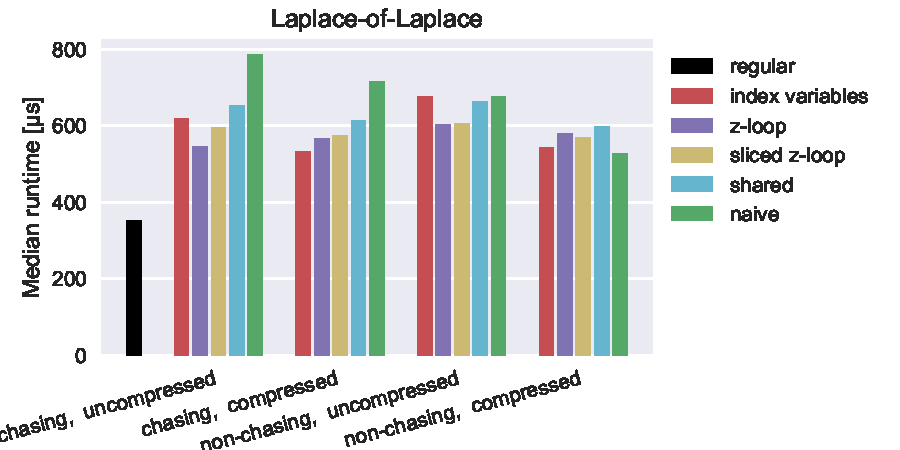
\includegraphics[scale=0.75]{overview-laplap.pdf}
	
	\vspace{0.5cm}
	
	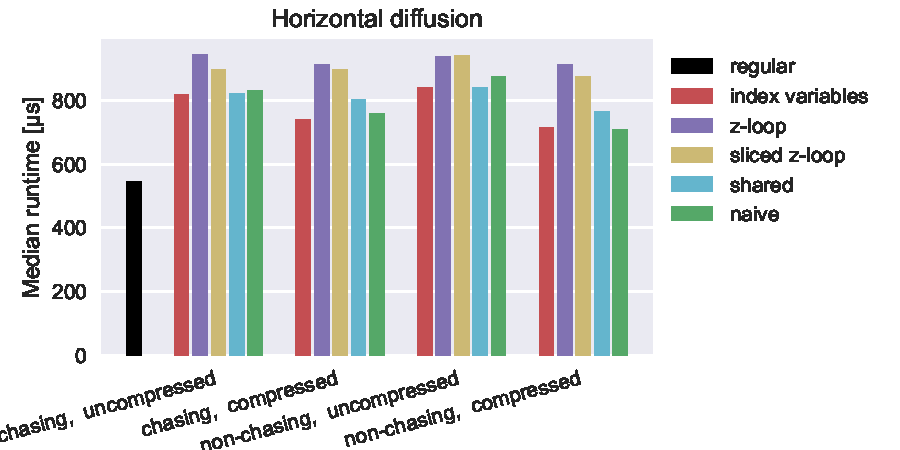
\includegraphics[scale=0.75]{overview-hdiff.pdf}
	
	\vspace{0.5cm}
	
	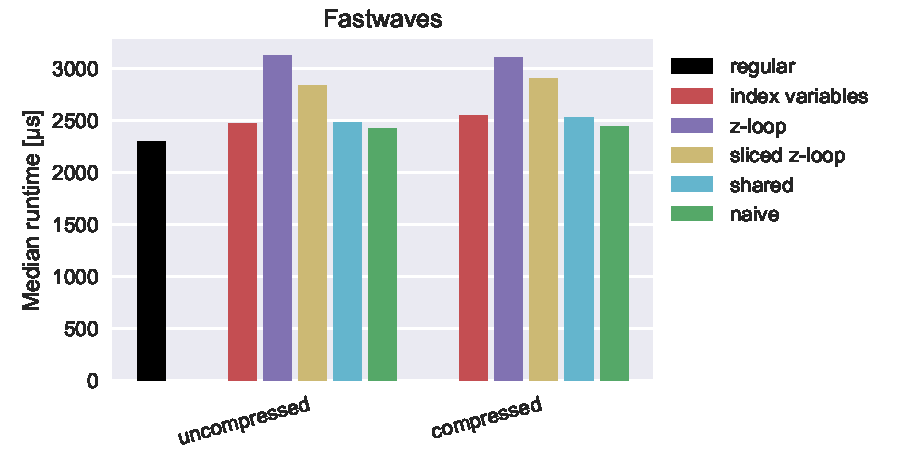
\includegraphics[scale=0.75]{overview-fastwaves.pdf}
	
	\caption{\label{fig:storage-access} Median runtimes across 20 runs for all combinations of storage and access strategy, for stencils on a $512\times512\times 64$-sized unstructured grid (z-curves layout).}
\end{figure}

Overall, we observed slowdowns around $50\%$, $30\%$ and $5\%$ compared to fastest regular grid performance for the \emph{laplap}, \emph{hdiff} and \emph{fastwaves} stencils, respectively. Figure \ref{fig:storage-access} shows an overview of the overhead for all tested combinations of storage and access strategy on a large grid of size $512\times 512\times 64$. For different domain sizes, see \ref{sec:res-size}. We chose to display the results for a \emph{z-curve} layout, but results for the \emph{row-major} benchmarks are similar. The fastest block size is plotted for each bar; for a more detailed analysis of what block sizes are beneficial to the different access strategies, see section \ref{sec:res-blocksize}. A more in-depth analysis of the different storage and access strategies is given in section \ref{sec:res-storage} and \ref{sec:res-access} respectively.